\documentclass[12pt,a4paper]{article}
\usepackage{graphicx}
\usepackage{float}
\usepackage[utf8]{vietnam}
\usepackage{geometry}
\usepackage{hyperref}
\usepackage{enumitem}
\geometry{
    a4paper,
    margin=1in
}

\setlist[itemize]{leftmargin=1.5cm}
\setlist[enumerate]{leftmargin=1.5cm}

\title{\textbf{PHÂN TÍCH NGƯỜI DÙNG VÀ USECASE}\\
\Large ĐỒ ÁN 1 (15/10/2026)}
\author{\textbf{Đề tài:} Xây dựng website thương mại điện tử\\
bán máy tính và linh kiện máy tính}

\date{}

\begin{document}

\maketitle
\section{PHẠM VI HỆ THỐNG}

Hệ thống được xây dựng nhằm hỗ trợ hoạt động kinh doanh máy tính và linh kiện máy tính thông qua website thương mại điện tử. Người dùng có thể xem, tìm kiếm và lựa chọn sản phẩm, quản lý giỏ hàng, đặt hàng và thanh toán. Hệ thống cũng hỗ trợ quản lý đơn hàng, sản phẩm, danh mục, người dùng, kho và thống kê.

Phạm vi của hệ thống tập trung vào các chức năng cốt lõi, phù hợp với thời gian thực hiện Đồ án 1. Các chức năng nâng cao như AI, chatbot, đa nhà bán hàng, tích điểm, voucher, đánh giá sản phẩm và hệ thống vận chuyển phức tạp không thuộc phạm vi hiện tại.

\section{PHÂN TÍCH NGƯỜI DÙNG (ACTOR)}

\begin{itemize}

 \item \textbf{Khách vãng lai:} Là người truy cập website nhưng chưa được xác thực đăng nhập vào hệ thống. Khách vãng lai có thể đã có hoặc chưa có tài khoản. Actor này có thể đăng ký, đăng nhập, xem, tìm kiếm và lọc sản phẩm.

 \item \textbf{Khách hàng:} Là người đã có tài khoản và đăng nhập vào hệ thống. Khách hàng có thể xem sản phẩm, quản lý giỏ hàng, đặt hàng, thanh toán, theo dõi và hủy đơn hàng theo điều kiện cho phép, đồng thời quản lý thông tin tài khoản.

 \item \textbf{Nhân viên:} Là người hỗ trợ hoạt động bán hàng và xử lý đơn hàng. Nhân viên có thể xem và xử lý đơn hàng trong phạm vi quyền được cấp, đồng thời kiểm tra số lượng tồn kho của sản phẩm. Nhân viên không có quyền trực tiếp điều chỉnh tồn kho.

 \item \textbf{Quản trị viên:} Là người có quyền quản lý và vận hành hệ thống. Quản trị viên có thể quản lý đơn hàng, sản phẩm, danh mục, người dùng, kho và xem các số liệu thống kê.

 \item \textbf{Cổng thanh toán:} Là hệ thống bên ngoài được sử dụng để xử lý các giao dịch thanh toán trực tuyến và trả kết quả giao dịch về cho hệ thống.

\end{itemize}

\section{DANH SÁCH USE CASE CHÍNH}

\begin{itemize}
    \item \textbf{UC01: Đăng ký}
    \item \textbf{UC02: Đăng nhập}
    \item \textbf{UC03: Xem, tìm kiếm và lọc sản phẩm}
    \item \textbf{UC04: Quản lý giỏ hàng}
    \item \textbf{UC05: Đặt hàng}
    \item \textbf{UC06: Thanh toán}
    \item \textbf{UC07: Theo dõi và hủy đơn hàng}
    \item \textbf{UC08: Quản lý tài khoản}
    \item \textbf{UC09: Quản lý đơn hàng}
    \item \textbf{UC10: Kiểm tra tồn kho}
    \item \textbf{UC11: Quản lý sản phẩm}
    \item \textbf{UC12: Quản lý danh mục}
    \item \textbf{UC13: Quản lý người dùng}
    \item \textbf{UC14: Quản lý kho}
    \item \textbf{UC15: Xem thống kê}
\end{itemize}

\section{QUY TRÌNH NGHIỆP VỤ CHUNG}

\subsection*{Quy trình xử lý đơn hàng}

Quy trình xử lý đơn hàng trong hệ thống được xác định như sau:

\begin{center}
Chờ xác nhận $\rightarrow$ Đang chuẩn bị hàng $\rightarrow$ Đang giao hàng $\rightarrow$ Hoàn thành
\end{center}

Ngoài luồng xử lý chính, đơn hàng có thể chuyển từ trạng thái \textbf{Chờ xác nhận} sang \textbf{Đã hủy} khi khách hàng thực hiện hủy đơn theo điều kiện cho phép.

\subsection*{Quy tắc chuyển trạng thái đơn hàng}
\begin{itemize}
    \item \textbf{Chờ xác nhận $\rightarrow$ Đang chuẩn bị hàng:} Nhân viên hoặc Quản trị viên xác nhận đơn hàng sau khi kiểm tra thông tin và tồn kho hợp lệ.
    \item \textbf{Chờ xác nhận $\rightarrow$ Đã hủy:} Khách hàng được phép hủy đơn khi đơn hàng chưa được xác nhận.
    \item \textbf{Đang chuẩn bị hàng $\rightarrow$ Đang giao hàng:} Đơn hàng đã được chuẩn bị và chuyển sang quá trình giao hàng.
    \item \textbf{Đang giao hàng $\rightarrow$ Hoàn thành:} Đơn hàng hoàn tất quá trình giao hàng.
    \item Không cho phép chuyển trạng thái tùy ý; trạng thái mới phải phù hợp với quy trình xử lý đơn hàng.
    \item Đơn hàng đã ở trạng thái \textbf{Đã hủy} hoặc \textbf{Hoàn thành} không được chuyển sang trạng thái xử lý khác.
\end{itemize}

\subsection*{Quy tắc hủy đơn hàng}
\begin{itemize}
    \item Khách hàng chỉ được phép hủy đơn khi đơn hàng đang ở trạng thái \textbf{Chờ xác nhận}.
    \item Khách hàng không được phép tự hủy đơn khi đơn hàng đang ở trạng thái \textbf{Đang chuẩn bị hàng}, \textbf{Đang giao hàng} hoặc \textbf{Hoàn thành}.
    \item Đơn hàng đã ở trạng thái \textbf{Đã hủy} không thể thực hiện thao tác hủy lại.
\end{itemize}

\subsection*{Quy tắc quản lý tồn kho}
\begin{itemize}
    \item Khi khách hàng đặt hàng, hệ thống tạo đơn hàng nhưng chưa trừ số lượng tồn kho.
    \item Khi Nhân viên hoặc Quản trị viên xác nhận đơn hàng, hệ thống phải kiểm tra lại số lượng tồn kho tại thời điểm xác nhận.
    \item Chỉ khi số lượng tồn kho đáp ứng đủ số lượng sản phẩm trong đơn, hệ thống mới cho phép xác nhận đơn và cập nhật số lượng tồn kho.
    \item Nếu số lượng tồn kho không đủ, hệ thống không cho phép xác nhận đơn hàng và thông báo cho người xử lý.
    \item Trong trường hợp nhiều đơn hàng cùng yêu cầu một sản phẩm nhưng số lượng tồn kho không đủ để đáp ứng tất cả, đơn hàng được xác nhận hợp lệ trước sẽ được cập nhật tồn kho trước; các đơn hàng xác nhận sau phải được kiểm tra lại tồn kho.
    \item Hệ thống không cho phép số lượng tồn kho nhỏ hơn 0.
    \item Khi khách hàng hủy đơn ở trạng thái \textbf{Chờ xác nhận}, hệ thống không cần hoàn lại tồn kho vì tồn kho chưa được trừ.
    \item Việc kiểm tra và cập nhật tồn kho khi xác nhận đơn phải bảo đảm không phát sinh tình trạng nhiều đơn hàng cùng sử dụng một số lượng tồn kho.
\end{itemize}

\subsection*{Quy tắc thanh toán}

Hệ thống hỗ trợ hai phương thức thanh toán cơ bản:

\begin{itemize}
    \item \textbf{Thanh toán khi nhận hàng (COD):} Khi đơn hàng được tạo, trạng thái thanh toán được ghi nhận là \textbf{Chưa thanh toán}. Khách hàng thực hiện thanh toán khi nhận hàng. Khi giao dịch COD được hoàn tất thành công, trạng thái thanh toán của đơn hàng được cập nhật thành \textbf{Đã thanh toán}.

    \item \textbf{Thanh toán trực tuyến:} Hệ thống gửi yêu cầu giao dịch đến Cổng thanh toán. Chỉ khi nhận được kết quả giao dịch hợp lệ và thành công, hệ thống mới cập nhật trạng thái thanh toán thành \textbf{Đã thanh toán}.
\end{itemize}

Trạng thái thanh toán gồm:

\begin{itemize}
    \item \textbf{Chưa thanh toán:} Đơn hàng chưa ghi nhận thanh toán thành công.
    \item \textbf{Đã thanh toán:} Đơn hàng đã ghi nhận thanh toán thành công.
\end{itemize}

\subsection*{Quy tắc xử lý thanh toán trực tuyến thất bại}

\begin{itemize}
    \item Nếu giao dịch trực tuyến thất bại hoặc bị khách hàng hủy, hệ thống giữ trạng thái thanh toán là \textbf{Chưa thanh toán} và thông báo kết quả cho khách hàng.

    \item Đối với đơn hàng vẫn còn hiệu lực và đang ở trạng thái chưa thanh toán, khách hàng được phép thực hiện lại thao tác thanh toán trực tuyến.

    \item Hệ thống không tự động chuyển trạng thái thanh toán thành \textbf{Đã thanh toán} nếu chưa nhận được kết quả giao dịch thành công hợp lệ từ Cổng thanh toán.

    \item Đơn hàng đã ở trạng thái \textbf{Đã thanh toán} không được thực hiện thanh toán lại.

    \item Đơn hàng đã ở trạng thái \textbf{Đã hủy} không được thực hiện thanh toán.

    \item Việc chuyển đổi từ thanh toán trực tuyến sang COD chỉ được thực hiện nếu hệ thống có hỗ trợ chức năng thay đổi phương thức thanh toán.
\end{itemize}

\section{ĐẶC TẢ CHI TIẾT CÁC USE CASE}

% ==================================================

\subsection*{UC01. Đăng ký}

\begin{itemize}
    \item \textbf{Actor:} Khách vãng lai.
    \item \textbf{Mục tiêu:} Cho phép khách vãng lai tạo tài khoản mới để sử dụng các chức năng dành cho khách hàng.
    \item \textbf{Mô tả:} Use Case này cho phép người dùng chưa đăng nhập đăng ký tài khoản mới bằng cách cung cấp các thông tin cần thiết. Hệ thống kiểm tra tính đầy đủ, hợp lệ và tính duy nhất của thông tin trước khi tạo tài khoản.
    \item \textbf{Điều kiện trước:} Người dùng chưa đăng nhập vào hệ thống.
    \item \textbf{Luồng chính:}
    \begin{enumerate}
        \item Người dùng chọn chức năng Đăng ký.
        \item Hệ thống hiển thị biểu mẫu đăng ký.
        \item Người dùng nhập các thông tin cần thiết.
        \item Người dùng gửi thông tin đăng ký.
        \item Hệ thống kiểm tra tính đầy đủ và hợp lệ của thông tin.
        \item Hệ thống kiểm tra tài khoản đã tồn tại hay chưa.
        \item Hệ thống tạo tài khoản mới.
        \item Hệ thống thông báo đăng ký thành công.
    \end{enumerate}
    \item \textbf{Luồng thay thế / Ngoại lệ:}
    \begin{itemize}
        \item Nếu thông tin chưa đầy đủ, hệ thống thông báo và yêu cầu người dùng bổ sung thông tin.
        \item Nếu thông tin không hợp lệ, hệ thống thông báo lỗi và yêu cầu người dùng kiểm tra, nhập lại thông tin.
        \item Nếu tài khoản đã tồn tại, hệ thống thông báo tài khoản đã tồn tại và yêu cầu người dùng sử dụng thông tin khác.
    \end{itemize}
    \item \textbf{Điều kiện sau:} Tài khoản mới được tạo thành công.
    \item \textbf{Quy tắc nghiệp vụ:}
    \begin{itemize}
        \item Thông tin đăng ký phải đầy đủ và hợp lệ.
        \item Thông tin định danh tài khoản không được trùng với tài khoản đã tồn tại.
    \end{itemize}
\end{itemize}

% ==================================================

\subsection*{UC02. Đăng nhập}

\begin{itemize}
    \item \textbf{Actor:} Khách vãng lai.
    \item \textbf{Mục tiêu:} Cho phép người dùng xác thực tài khoản và đăng nhập vào hệ thống.
    \item \textbf{Mô tả:} Use Case này cho phép người dùng cung cấp thông tin đăng nhập. Hệ thống kiểm tra thông tin xác thực và trạng thái tài khoản trước khi thiết lập trạng thái đăng nhập.
    \item \textbf{Điều kiện trước:} Người dùng chưa đăng nhập vào hệ thống.
    \item \textbf{Luồng chính:}
    \begin{enumerate}
        \item Người dùng chọn chức năng Đăng nhập.
        \item Hệ thống hiển thị biểu mẫu đăng nhập.
        \item Người dùng nhập thông tin đăng nhập.
        \item Người dùng gửi thông tin đăng nhập.
        \item Hệ thống kiểm tra thông tin đăng nhập.
        \item Hệ thống kiểm tra trạng thái tài khoản.
        \item Hệ thống thiết lập trạng thái đăng nhập.
        \item Hệ thống thông báo đăng nhập thành công.
    \end{enumerate}
    \item \textbf{Luồng thay thế / Ngoại lệ:}
    \begin{itemize}
        \item Nếu thông tin đăng nhập chưa đầy đủ, hệ thống thông báo dữ liệu chưa đầy đủ và yêu cầu người dùng nhập lại.
        \item Nếu tài khoản không tồn tại, hệ thống thông báo tài khoản không tồn tại và cho phép người dùng chuyển sang UC01 -- Đăng ký.
        \item Nếu mật khẩu không chính xác, hệ thống thông báo mật khẩu không đúng và yêu cầu người dùng nhập lại.
        \item Nếu tài khoản ở trạng thái \textbf{Không còn hoạt động}, hệ thống thông báo tài khoản không tồn tại và từ chối đăng nhập.
        \item Nếu tài khoản ở trạng thái \textbf{Bị vô hiệu hóa}, hệ thống thông báo tài khoản đã bị vô hiệu hóa và từ chối đăng nhập.
        \item Nếu không thể thiết lập trạng thái đăng nhập, hệ thống thông báo xảy ra lỗi trong quá trình đăng nhập và yêu cầu người dùng thực hiện lại.
    \end{itemize}
    \item \textbf{Điều kiện sau:} Người dùng được xác thực và đăng nhập thành công; trạng thái đăng nhập được thiết lập.
    \item \textbf{Quy tắc nghiệp vụ:}
    \begin{itemize}
        \item Chỉ tài khoản tồn tại và đang ở trạng thái \textbf{Hoạt động} mới được phép đăng nhập.
        \item Tài khoản bị vô hiệu hóa hoặc không còn hoạt động không được phép đăng nhập.
    \end{itemize}
\end{itemize}

% ==================================================

\subsection*{UC03. Xem, tìm kiếm và lọc sản phẩm}

\begin{itemize}

 \item \textbf{Actor:} Khách vãng lai, Khách hàng.

 \item \textbf{Mục tiêu:} Cho phép người dùng tra cứu và xem thông tin sản phẩm phù hợp với nhu cầu.

 \item \textbf{Mô tả:} Use Case này cho phép người dùng xem danh sách sản phẩm mà không cần đăng nhập. Người dùng có thể tìm kiếm sản phẩm bằng từ khóa, lựa chọn danh mục, lọc theo khoảng giá hoặc thương hiệu. Sau khi tìm được sản phẩm phù hợp, người dùng có thể xem thông tin chi tiết như tên, hình ảnh, giá bán, mô tả, thông số kỹ thuật và tình trạng tồn kho.

 \item \textbf{Điều kiện trước:} Sản phẩm tồn tại và đang được phép hiển thị trên website.

 \item \textbf{Luồng chính:}

 \begin{enumerate}

  \item Người dùng truy cập khu vực hiển thị sản phẩm.

  \item Hệ thống hiển thị danh sách sản phẩm đang kinh doanh.

  \item Người dùng có thể chọn danh mục sản phẩm.

  \item Người dùng có thể nhập từ khóa tìm kiếm.

  \item Người dùng có thể lọc sản phẩm theo khoảng giá hoặc thương hiệu.

  \item Hệ thống xử lý yêu cầu và hiển thị kết quả phù hợp.

  \item Người dùng chọn một sản phẩm.

  \item Hệ thống hiển thị thông tin chi tiết của sản phẩm.

 \end{enumerate}

 \item \textbf{Luồng thay thế / Ngoại lệ:}

 \begin{itemize}

  \item Nếu không tìm thấy sản phẩm phù hợp, hệ thống thông báo hoặc hiển thị danh sách kết quả trống.

  \item Sản phẩm ngừng kinh doanh không được hiển thị trong danh sách sản phẩm dành cho khách hàng.

  \item Sản phẩm hết hàng vẫn có thể được hiển thị nhưng phải thể hiện rõ tình trạng hết hàng.

 \end{itemize}

 \item \textbf{Điều kiện sau:} Người dùng nhận được danh sách hoặc thông tin chi tiết của sản phẩm.

 \item \textbf{Quy tắc nghiệp vụ:}

 \begin{itemize}

  \item Không yêu cầu đăng nhập để xem, tìm kiếm và lọc sản phẩm.

  \item Chỉ sản phẩm đang được phép kinh doanh mới được hiển thị trong danh sách thông thường.

  \item Thông tin sản phẩm hiển thị phải phù hợp với dữ liệu hiện có trong hệ thống.

 \end{itemize}

\end{itemize}

% ==================================================

\subsection*{UC04. Quản lý giỏ hàng}

\begin{itemize}

 \item \textbf{Actor:} Khách hàng.

 \item \textbf{Mục tiêu:} Cho phép khách hàng quản lý các sản phẩm dự định mua.

 \item \textbf{Mô tả:} Use Case này cho phép khách hàng thêm sản phẩm vào giỏ hàng, thay đổi số lượng hoặc xóa sản phẩm không còn nhu cầu mua. Giỏ hàng được quản lý theo tài khoản của khách hàng nên người dùng phải đăng nhập để hệ thống xác định chính xác giỏ hàng thuộc tài khoản nào. Hệ thống kiểm tra tình trạng sản phẩm và cập nhật thông tin giỏ hàng tương ứng với các thao tác của khách hàng.

 \item \textbf{Điều kiện trước:}
    \begin{itemize}
        \item Khách hàng đã đăng nhập.
        \item Giỏ hàng thuộc tài khoản của khách hàng đang đăng nhập.
    \end{itemize}

 \item \textbf{Luồng chính:}

 \begin{enumerate}

  \item Khách hàng chọn sản phẩm.

  \item Khách hàng thêm sản phẩm vào giỏ hàng.

  \item Hệ thống cập nhật giỏ hàng.

  \item Khách hàng có thể thay đổi số lượng hoặc xóa sản phẩm.

  \item Hệ thống cập nhật lại thông tin và tổng tiền của giỏ hàng.

 \end{enumerate}

 \item \textbf{Luồng thay thế / Ngoại lệ:} Nếu sản phẩm ngừng kinh doanh hoặc không còn hàng, hệ thống không cho phép thêm sản phẩm vào giỏ hàng.

 \item \textbf{Điều kiện sau:} Giỏ hàng được cập nhật theo thao tác của khách hàng.

 \item \textbf{Quy tắc nghiệp vụ:}

 \begin{itemize}

  \item Số lượng sản phẩm trong giỏ phải lớn hơn 0.

  \item Không cho phép thêm sản phẩm ngừng kinh doanh vào giỏ hàng.

 \end{itemize}

\end{itemize}

% ==================================================

\subsection*{UC05. Đặt hàng}

\begin{itemize}

 \item \textbf{Actor:} Khách hàng.

 \item \textbf{Mục tiêu:} Tạo đơn hàng từ các sản phẩm trong giỏ hàng.

 \item \textbf{Mô tả:} Use Case này cho phép khách hàng tạo đơn hàng từ các sản phẩm đã chọn trong giỏ hàng. Khách hàng kiểm tra lại thông tin sản phẩm, số lượng, tổng tiền, cung cấp thông tin nhận hàng và lựa chọn phương thức thanh toán cho đơn hàng. Hệ thống kiểm tra thông tin trước khi tạo đơn hàng với trạng thái ban đầu là \textbf{Chờ xác nhận}. Việc xử lý thanh toán được thực hiện riêng trong UC06 -- Thanh toán.

 \item \textbf{Điều kiện trước:} Khách hàng đã đăng nhập và giỏ hàng có ít nhất một sản phẩm.

 \item \textbf{Luồng chính:}

 \begin{enumerate}

  \item Khách hàng truy cập giỏ hàng.

  \item Khách hàng chọn chức năng Đặt hàng.

  \item Hệ thống hiển thị thông tin sản phẩm và tổng tiền.

  \item Khách hàng nhập hoặc chọn thông tin nhận hàng.

  \item Khách hàng lựa chọn phương thức thanh toán.

  \item Hệ thống kiểm tra thông tin.

  \item Khách hàng xác nhận đặt hàng.

  \item Hệ thống tạo đơn hàng với trạng thái Chờ xác nhận.

 \end{enumerate}

 \item \textbf{Luồng thay thế / Ngoại lệ:} Nếu thông tin nhận hàng không hợp lệ hoặc giỏ hàng không còn sản phẩm hợp lệ, hệ thống thông báo và yêu cầu khách hàng điều chỉnh.

 \item \textbf{Điều kiện sau:} Đơn hàng được tạo với trạng thái \textbf{Chờ xác nhận}.

 \item \textbf{Quy tắc nghiệp vụ:}

 \begin{itemize}

  \item Nếu thông tin nhận hàng không hợp lệ, hệ thống thông báo và yêu cầu khách hàng điều chỉnh.

  \item Nếu giỏ hàng không còn sản phẩm hợp lệ, hệ thống thông báo và yêu cầu khách hàng cập nhật lại giỏ hàng.

  \item Nếu sản phẩm trong giỏ đã ngừng kinh doanh hoặc không còn khả dụng, hệ thống không cho phép tạo đơn hàng và yêu cầu khách hàng cập nhật lại giỏ hàng.

  \item Không tạo đơn hàng khi giỏ hàng trống.

  \item Việc đặt hàng và thanh toán là hai nghiệp vụ riêng biệt.

  \item Đặt hàng không làm giảm số lượng tồn kho ngay lập tức.

 \end{itemize}

\end{itemize}

% ==================================================

\subsection*{UC06. Thanh toán}

\begin{itemize}

 \item \textbf{Actor:} Khách hàng, Cổng thanh toán.

 \item \textbf{Mục tiêu:} Xử lý thanh toán cho đơn hàng.

 \item \textbf{Mô tả:} Use Case này cho phép khách hàng thực hiện thanh toán cho đơn hàng bằng phương thức thanh toán khi nhận hàng hoặc thanh toán trực tuyến. Đối với thanh toán khi nhận hàng, hệ thống ghi nhận trạng thái thanh toán là \textbf{Chưa thanh toán}. Đối với thanh toán trực tuyến, hệ thống gửi yêu cầu giao dịch đến Cổng thanh toán và cập nhật trạng thái thanh toán dựa trên kết quả trả về.

 \item \textbf{Điều kiện trước:} Đơn hàng đã được tạo, chưa bị hủy và đang ở trạng thái chưa thanh toán.

\item \textbf{Luồng chính:}

\begin{enumerate}

    \item Khách hàng truy cập chức năng thanh toán cho đơn hàng chưa thanh toán.

    \item Hệ thống kiểm tra trạng thái đơn hàng và trạng thái thanh toán.

    \item Hệ thống xác định phương thức thanh toán đã được lựa chọn khi đặt hàng.

    \item Nếu phương thức thanh toán là COD, hệ thống ghi nhận trạng thái thanh toán là \textbf{Chưa thanh toán}.

    \item Nếu phương thức thanh toán là trực tuyến, hệ thống tạo yêu cầu giao dịch.

    \item Hệ thống gửi yêu cầu đến Cổng thanh toán.

    \item Cổng thanh toán xử lý giao dịch và trả kết quả.

    \item Hệ thống kiểm tra kết quả giao dịch và cập nhật trạng thái thanh toán tương ứng.

\end{enumerate}

\item \textbf{Luồng thay thế / Ngoại lệ:}

\begin{itemize}

    \item Nếu giao dịch trực tuyến thất bại hoặc bị khách hàng hủy, hệ thống giữ trạng thái thanh toán là \textbf{Chưa thanh toán} và thông báo cho khách hàng.

    \item Nếu đơn hàng đã ở trạng thái \textbf{Đã thanh toán}, hệ thống từ chối thực hiện thanh toán lại.

    \item Nếu đơn hàng đã ở trạng thái \textbf{Đã hủy}, hệ thống từ chối thực hiện thanh toán.

    \item Nếu không nhận được kết quả giao dịch hợp lệ từ Cổng thanh toán, hệ thống không cập nhật trạng thái thành \textbf{Đã thanh toán}.

\end{itemize}

 \item \textbf{Điều kiện sau:} Trạng thái thanh toán được ghi nhận là \textbf{Chưa thanh toán} hoặc \textbf{Đã thanh toán}.

 \item \textbf{Quy tắc nghiệp vụ:}

 \begin{itemize}

  \item Chỉ xác nhận thanh toán trực tuyến thành công khi nhận được kết quả hợp lệ từ Cổng thanh toán.

  \item Đơn hàng đã được thanh toán không được thanh toán lại.

 \end{itemize}

\end{itemize}

% ==================================================

\subsection*{UC07. Theo dõi và hủy đơn hàng}

\begin{itemize}

 \item \textbf{Actor:} Khách hàng.

 \item \textbf{Mục tiêu:} Cho phép khách hàng theo dõi tình trạng đơn hàng và hủy đơn khi đáp ứng điều kiện.

 \item \textbf{Mô tả:} Use Case này cho phép khách hàng xem danh sách và thông tin chi tiết các đơn hàng thuộc tài khoản của mình. Khách hàng có thể theo dõi trạng thái xử lý và trạng thái thanh toán của từng đơn hàng. Khách hàng chỉ được phép yêu cầu hủy đơn khi đơn hàng đang ở trạng thái \textbf{Chờ xác nhận}. Khi đơn hàng đã được xác nhận và chuyển sang quá trình chuẩn bị hoặc giao hàng, khách hàng không được phép tự hủy đơn.

 \item \textbf{Điều kiện trước:}

 \begin{itemize}

  \item Khách hàng đã đăng nhập vào hệ thống.

  \item Đơn hàng tồn tại trong hệ thống.

  \item Đơn hàng thuộc tài khoản của khách hàng đang đăng nhập.

 \end{itemize}

 \item \textbf{Luồng chính:}

 \begin{enumerate}

  \item Khách hàng chọn một đơn hàng để xem chi tiết.

  \item Hệ thống hiển thị thông tin đơn hàng, trạng thái xử lý và trạng thái thanh toán.

  \item Nếu đơn hàng đang ở trạng thái \textbf{Chờ xác nhận}, hệ thống hiển thị chức năng hủy đơn.

  \item Khách hàng chọn chức năng hủy đơn.

  \item Hệ thống kiểm tra trạng thái đơn hàng.

  \item Hệ thống cập nhật trạng thái đơn hàng thành \textbf{Đã hủy}.

  \item Hệ thống thông báo kết quả cho khách hàng.

 \end{enumerate}

 \item \textbf{Luồng thay thế / Ngoại lệ:}

 \begin{itemize}

  \item Nếu đơn hàng không thuộc tài khoản của khách hàng, hệ thống từ chối truy cập.

  \item Nếu đơn hàng không còn ở trạng thái Chờ xác nhận, hệ thống không cho phép hủy.

  \item Nếu đơn hàng đã bị hủy hoặc không tồn tại, hệ thống thông báo trạng thái phù hợp.

 \end{itemize}

 \item \textbf{Điều kiện sau:} Thông tin đơn hàng được hiển thị hoặc trạng thái đơn hàng được cập nhật thành \textbf{Đã hủy}.

 \item \textbf{Quy tắc nghiệp vụ:}

\begin{itemize}

    \item Khách hàng chỉ được xem đơn hàng thuộc tài khoản của mình.

    \item Khách hàng chỉ được hủy đơn khi đơn hàng đang ở trạng thái \textbf{Chờ xác nhận}.

    \item Đơn hàng từ trạng thái \textbf{Đang chuẩn bị hàng} trở đi không được khách hàng tự hủy.

    \item Đơn hàng đã ở trạng thái \textbf{Đã hủy} không thể thực hiện thao tác hủy lại.

\end{itemize}

\end{itemize}

% ==================================================

\subsection*{UC08. Quản lý tài khoản}

\begin{itemize}

 \item \textbf{Actor:} Khách hàng.

 \item \textbf{Mục tiêu:} Cho phép khách hàng quản lý thông tin tài khoản.

 \item \textbf{Mô tả:} Use Case này cho phép khách hàng xem và cập nhật các thông tin liên quan đến tài khoản của mình, bao gồm thông tin cá nhân, thông tin liên hệ, địa chỉ nhận hàng và mật khẩu. Hệ thống kiểm tra tính hợp lệ của dữ liệu trước khi lưu thay đổi.

 \item \textbf{Điều kiện trước:} Khách hàng đã đăng nhập.

 \item \textbf{Luồng chính:}

 \begin{enumerate}

  \item Khách hàng truy cập thông tin tài khoản.

  \item Hệ thống hiển thị thông tin hiện có.

  \item Khách hàng chỉnh sửa thông tin hoặc thay đổi mật khẩu.

  \item Hệ thống kiểm tra dữ liệu.

  \item Hệ thống lưu thay đổi.

 \end{enumerate}

 \item \textbf{Luồng thay thế / Ngoại lệ:} Nếu thông tin không hợp lệ hoặc mật khẩu hiện tại không chính xác, hệ thống thông báo và không lưu thay đổi.

 \item \textbf{Điều kiện sau:} Thông tin tài khoản được cập nhật.

\end{itemize}

% ==================================================

\subsection*{UC09. Quản lý đơn hàng}

\begin{itemize}
    \item \textbf{Actor:} Nhân viên, Quản trị viên.
    \item \textbf{Mục tiêu:} Theo dõi và xử lý các đơn hàng trong hệ thống.
    \item \textbf{Mô tả:} Use Case này cho phép Nhân viên và Quản trị viên xem danh sách, kiểm tra thông tin và xử lý đơn hàng theo quyền được cấp. Khi đơn hàng ở trạng thái \textbf{Chờ xác nhận}, người xử lý kiểm tra thông tin và tồn kho trước khi xác nhận đơn. Sau khi xác nhận thành công, hệ thống cập nhật số lượng tồn kho và chuyển đơn hàng sang trạng thái \textbf{Đang chuẩn bị hàng}. Đơn hàng tiếp tục được cập nhật theo quy trình xử lý cho đến khi hoàn thành.
    \item \textbf{Phân quyền:}
\end{itemize}

\begin{center}
\begin{tabular}{|p{7cm}|c|c|}
\hline
\textbf{Thao tác} & \textbf{Nhân viên} & \textbf{Quản trị viên} \\
\hline
Xem danh sách đơn hàng & Có & Có \\
\hline
Xem chi tiết đơn hàng & Có & Có \\
\hline
Kiểm tra tồn kho khi xử lý đơn & Có & Có \\
\hline
Xác nhận đơn hàng & Có & Có \\
\hline
Cập nhật trạng thái xử lý đơn & Có & Có \\
\hline
Quản lý toàn bộ đơn hàng & Không & Có \\
\hline
\end{tabular}
\end{center}

\begin{itemize}
    \item \textbf{Điều kiện trước:} Nhân viên hoặc Quản trị viên đã đăng nhập và có quyền xử lý đơn hàng.
    \item \textbf{Luồng chính:}
    \begin{enumerate}
        \item Người dùng truy cập danh sách đơn hàng.
        \item Hệ thống kiểm tra quyền và hiển thị các đơn hàng theo phạm vi quyền.
        \item Người dùng chọn một đơn hàng để xem chi tiết.
        \item Người dùng kiểm tra thông tin đơn hàng.
        \item Nếu đơn hàng đang ở trạng thái Chờ xác nhận, người dùng kiểm tra số lượng tồn kho.
        \item Hệ thống kiểm tra lại số lượng tồn kho tại thời điểm xác nhận.
        \item Người dùng xác nhận đơn hàng.
        \item Hệ thống cập nhật số lượng tồn kho tương ứng.
        \item Hệ thống chuyển đơn hàng sang trạng thái Đang chuẩn bị hàng.
        \item Người dùng tiếp tục cập nhật trạng thái đơn hàng theo quy trình xử lý.
        \item Hệ thống lưu các thay đổi.
    \end{enumerate}
    \item \textbf{Luồng thay thế / Ngoại lệ:}
    \begin{itemize}
        \item Nếu người dùng không có quyền thực hiện thao tác, hệ thống từ chối thao tác.
        \item Nếu sản phẩm không đủ tồn kho tại thời điểm xác nhận, hệ thống không cho phép xác nhận đơn.
        \item Nếu đơn hàng đã được xử lý bởi người dùng khác trước đó, hệ thống kiểm tra lại trạng thái và tồn kho trước khi tiếp tục thao tác.
        \item Nếu trạng thái hiện tại không cho phép chuyển sang trạng thái tiếp theo, hệ thống từ chối cập nhật.
    \end{itemize}
    \item \textbf{Điều kiện sau:} Thông tin và trạng thái đơn hàng được cập nhật theo thao tác hợp lệ; nếu đơn được xác nhận thành công, số lượng tồn kho được cập nhật tương ứng.
    \item \textbf{Quy tắc nghiệp vụ:}
    \begin{itemize}
        \item Nhân viên chỉ được thực hiện các thao tác trong phạm vi quyền được cấp.
        \item Quản trị viên có quyền theo dõi và quản lý toàn bộ đơn hàng.
        \item Số lượng tồn kho chỉ được cập nhật khi đơn hàng được xác nhận thành công và tồn kho đủ.
        \item Trạng thái đơn hàng phải tuân theo quy trình đã xác định.
    \end{itemize}
\end{itemize}

% ==================================================

\subsection*{UC10. Kiểm tra tồn kho}

\begin{itemize}

 \item \textbf{Actor:} Nhân viên.

 \item \textbf{Mục tiêu:} Tra cứu số lượng sản phẩm còn trong kho để hỗ trợ xử lý đơn hàng.

 \item \textbf{Mô tả:} Use Case này cho phép Nhân viên tra cứu số lượng tồn kho của từng sản phẩm. Nhân viên có thể tìm kiếm hoặc chọn sản phẩm cần kiểm tra, sau đó hệ thống hiển thị số lượng tồn kho hiện tại. Chức năng này chỉ phục vụ việc tra cứu và không cho phép Nhân viên tự ý điều chỉnh số lượng kho.

 \item \textbf{Điều kiện trước:} Nhân viên đã đăng nhập.

 \item \textbf{Luồng chính:}

 \begin{enumerate}

  \item Nhân viên truy cập chức năng kiểm tra tồn kho.

  \item Nhân viên nhập hoặc chọn sản phẩm.

  \item Hệ thống truy xuất thông tin tồn kho.

  \item Hệ thống hiển thị số lượng hiện có.

 \end{enumerate}

 \item \textbf{Luồng thay thế / Ngoại lệ:} Nếu không tìm thấy sản phẩm, hệ thống thông báo cho Nhân viên.

 \item \textbf{Điều kiện sau:} Thông tin tồn kho được hiển thị.

 \item \textbf{Quy tắc nghiệp vụ:} Nhân viên chỉ có quyền tra cứu tồn kho, không có quyền trực tiếp điều chỉnh số lượng tồn kho.

\end{itemize}

% ==================================================

\subsection*{UC11. Quản lý sản phẩm}

\begin{itemize}

 \item \textbf{Actor:} Quản trị viên.

 \item \textbf{Mục tiêu:} Quản lý thông tin các sản phẩm được kinh doanh trên hệ thống.

 \item \textbf{Mô tả:} Use Case này cho phép Quản trị viên thêm mới, chỉnh sửa và cập nhật trạng thái kinh doanh của sản phẩm. Các thông tin được quản lý bao gồm tên sản phẩm, giá bán, hình ảnh, mô tả, danh mục, thương hiệu và thông số kỹ thuật. Chức năng này không trực tiếp quản lý số lượng tồn kho.

 \item \textbf{Điều kiện trước:} Quản trị viên đã đăng nhập.

 \item \textbf{Luồng chính:}

 \begin{enumerate}

  \item Quản trị viên truy cập chức năng quản lý sản phẩm.

  \item Hệ thống hiển thị danh sách sản phẩm.

  \item Quản trị viên chọn thêm mới, chỉnh sửa hoặc cập nhật trạng thái sản phẩm.

  \item Quản trị viên nhập hoặc chỉnh sửa thông tin.

  \item Hệ thống kiểm tra dữ liệu.

  \item Hệ thống lưu thay đổi.

 \end{enumerate}

 \item \textbf{Luồng thay thế / Ngoại lệ:} Nếu thông tin không hợp lệ, hệ thống thông báo và yêu cầu chỉnh sửa.

 \item \textbf{Điều kiện sau:} Thông tin hoặc trạng thái sản phẩm được cập nhật.

 \item \textbf{Quy tắc nghiệp vụ:}

 \begin{itemize}

  \item Sản phẩm có thể ở trạng thái Đang kinh doanh hoặc Ngừng kinh doanh.

  \item Sản phẩm đã phát sinh trong đơn hàng không được xóa vật lý khỏi hệ thống; khi không còn kinh doanh, sản phẩm phải được chuyển sang trạng thái Ngừng kinh doanh.

  \item Số lượng tồn kho được quản lý trong UC14.

 \end{itemize}

\end{itemize}

% ==================================================

\subsection*{UC12. Quản lý danh mục}

\begin{itemize}

 \item \textbf{Actor:} Quản trị viên.

 \item \textbf{Mục tiêu:} Quản lý việc phân loại sản phẩm.

 \item \textbf{Mô tả:} Use Case này cho phép Quản trị viên thêm mới, chỉnh sửa hoặc cập nhật thông tin các danh mục sản phẩm. Danh mục được sử dụng để phân loại và hỗ trợ người dùng tìm kiếm sản phẩm trên website.

 \item \textbf{Điều kiện trước:} Quản trị viên đã đăng nhập.

 \item \textbf{Luồng chính:}

 \begin{enumerate}

  \item Quản trị viên truy cập chức năng quản lý danh mục.

  \item Hệ thống hiển thị danh sách danh mục.

  \item Quản trị viên thêm mới hoặc chỉnh sửa danh mục.

  \item Hệ thống kiểm tra dữ liệu.

  \item Hệ thống lưu thay đổi.

 \end{enumerate}

 \item \textbf{Luồng thay thế / Ngoại lệ:} Nếu tên danh mục đã tồn tại hoặc dữ liệu không hợp lệ, hệ thống thông báo và yêu cầu chỉnh sửa.

 \item \textbf{Điều kiện sau:} Danh mục được cập nhật.

 \item \textbf{Quy tắc nghiệp vụ:}

 \begin{itemize}

  \item Không được tạo danh mục trùng lặp.

  \item Không được xóa danh mục đang có sản phẩm liên kết.
        \item Nếu muốn xóa danh mục đang có sản phẩm liên kết, Quản trị viên phải chuyển các sản phẩm đó sang danh mục khác trước.
        \item Danh mục chỉ được xóa khi không còn sản phẩm liên kết.

 \end{itemize}

\end{itemize}

% ==================================================

\subsection*{UC13. Quản lý người dùng}

\begin{itemize}

 \item \textbf{Actor:} Quản trị viên.

 \item \textbf{Mục tiêu:} Quản lý tài khoản khách hàng và nhân viên trong hệ thống.

 \item \textbf{Mô tả:} Use Case này cho phép Quản trị viên xem, tìm kiếm và quản lý trạng thái các tài khoản trong hệ thống. Đối với tài khoản nhân viên, Quản trị viên có thể thêm mới hoặc cập nhật thông tin. Đối với tài khoản khách hàng, Quản trị viên có thể xem thông tin và khóa hoặc mở khóa tài khoản khi cần thiết. Trạng thái tài khoản được quản lý nhằm kiểm soát quyền đăng nhập và sử dụng hệ thống.

 \item \textbf{Điều kiện trước:} Quản trị viên đã đăng nhập.

 \item \textbf{Luồng chính:}

 \begin{enumerate}

  \item Quản trị viên truy cập chức năng quản lý người dùng.

  \item Hệ thống hiển thị danh sách tài khoản.

  \item Quản trị viên tìm kiếm hoặc chọn một tài khoản.

  \item Quản trị viên thực hiện thao tác phù hợp với loại tài khoản.

  \item Hệ thống kiểm tra quyền và dữ liệu.

  \item Hệ thống lưu thay đổi.

 \end{enumerate}

 \item \textbf{Luồng thay thế / Ngoại lệ:} Nếu dữ liệu không hợp lệ hoặc thao tác không được phép, hệ thống từ chối và thông báo.

 \item \textbf{Điều kiện sau:} Thông tin hoặc trạng thái tài khoản được cập nhật.

 \item \textbf{Quy tắc nghiệp vụ:}

 \begin{itemize}

  \item Tài khoản ở trạng thái \textbf{Hoạt động} được phép đăng nhập nếu thông tin xác thực hợp lệ.

  \item Tài khoản ở trạng thái \textbf{Bị vô hiệu hóa} không được phép đăng nhập cho đến khi được Quản trị viên mở khóa.

  \item Tài khoản ở trạng thái \textbf{Không còn hoạt động} không được phép đăng nhập.

  \item Không xóa cứng tài khoản đã liên quan đến dữ liệu giao dịch.

  \item Quản trị viên không được thực hiện thao tác làm mất quyền quản trị của tài khoản quản trị cuối cùng.

 \end{itemize}

\end{itemize}

% ==================================================

\subsection*{UC14. Quản lý kho}

\begin{itemize}

 \item \textbf{Actor:} Quản trị viên.

 \item \textbf{Mục tiêu:} Theo dõi và cập nhật số lượng hàng hóa trong kho.

 \item \textbf{Mô tả:} Use Case này cho phép Quản trị viên theo dõi số lượng tồn kho và thực hiện các thao tác nhập hoặc điều chỉnh số lượng sản phẩm khi cần thiết. Hệ thống kiểm tra dữ liệu trước khi cập nhật nhằm bảo đảm số lượng tồn kho chính xác và không nhỏ hơn 0.

 \item \textbf{Điều kiện trước:} Quản trị viên đã đăng nhập.

 \item \textbf{Luồng chính:}

 \begin{enumerate}

  \item Quản trị viên truy cập chức năng quản lý kho.

  \item Hệ thống hiển thị thông tin tồn kho.

  \item Quản trị viên chọn sản phẩm cần cập nhật.

  \item Quản trị viên thực hiện nhập kho hoặc điều chỉnh số lượng.

  \item Hệ thống kiểm tra dữ liệu.

  \item Hệ thống cập nhật số lượng tồn kho.

 \end{enumerate}

 \item \textbf{Luồng thay thế / Ngoại lệ:} Nếu số lượng cập nhật không hợp lệ hoặc thao tác làm tồn kho nhỏ hơn 0, hệ thống từ chối cập nhật.

 \item \textbf{Điều kiện sau:} Số lượng tồn kho được cập nhật.

 \item \textbf{Quy tắc nghiệp vụ:}

 \begin{itemize}

  \item Số lượng tồn kho không được nhỏ hơn 0.

  \item Mọi thay đổi tồn kho phải được kiểm tra trước khi lưu.

  \item Số lượng tồn kho không được cập nhật trực tiếp trong UC11.

  \item Mọi thay đổi tồn kho phải ghi nhận tối thiểu sản phẩm, số lượng thay đổi, loại thao tác, người thực hiện và thời gian thực hiện.

 \end{itemize}

\end{itemize}

% ==================================================

\subsection*{UC15. Xem thống kê}

\begin{itemize}

 \item \textbf{Actor:} Quản trị viên.

 \item \textbf{Mục tiêu:} Cung cấp số liệu tổng quan phục vụ quản lý hoạt động kinh doanh.

 \item \textbf{Mô tả:} Use Case này cho phép Quản trị viên xem các số liệu thống kê cơ bản như doanh thu, số lượng đơn hàng và tình hình sản phẩm. Quản trị viên có thể lựa chọn khoảng thời gian để hệ thống tổng hợp và hiển thị dữ liệu phù hợp.

 \item \textbf{Điều kiện trước:} Quản trị viên đã đăng nhập.

 \item \textbf{Luồng chính:}

 \begin{enumerate}

  \item Quản trị viên truy cập chức năng thống kê.

  \item Quản trị viên lựa chọn khoảng thời gian.

  \item Hệ thống tổng hợp dữ liệu liên quan.

  \item Hệ thống hiển thị kết quả thống kê.

 \end{enumerate}

 \item \textbf{Luồng thay thế / Ngoại lệ:} Nếu khoảng thời gian không hợp lệ hoặc không có dữ liệu, hệ thống hiển thị thông báo phù hợp.

 \item \textbf{Điều kiện sau:} Dữ liệu thống kê được hiển thị cho Quản trị viên.

 \item \textbf{Quy tắc nghiệp vụ:}
    \begin{itemize}
        \item Chỉ sử dụng dữ liệu hợp lệ hiện có trong hệ thống để thực hiện thống kê.
        \item Doanh thu chỉ được tính từ các đơn hàng ở trạng thái \textbf{Hoàn thành}.
        \item Đơn hàng ở trạng thái \textbf{Đã hủy} không được tính vào doanh thu.
        \item Đơn hàng ở trạng thái \textbf{Chờ xác nhận}, \textbf{Đang chuẩn bị hàng} và \textbf{Đang giao hàng} không được tính vào doanh thu thực tế.
    \end{itemize}

\end{itemize}

\newpage

\section{Biểu đồ Use Case tổng quát}

Biểu đồ Use Case tổng quát của hệ thống website T\&T COMPUTER

được sử dụng để mô tả các tác nhân bên ngoài và các chức năng

chính mà hệ thống cung cấp cho từng tác nhân.

\begin{figure}[H]

 \centering

 \IfFileExists{UseCase.png}{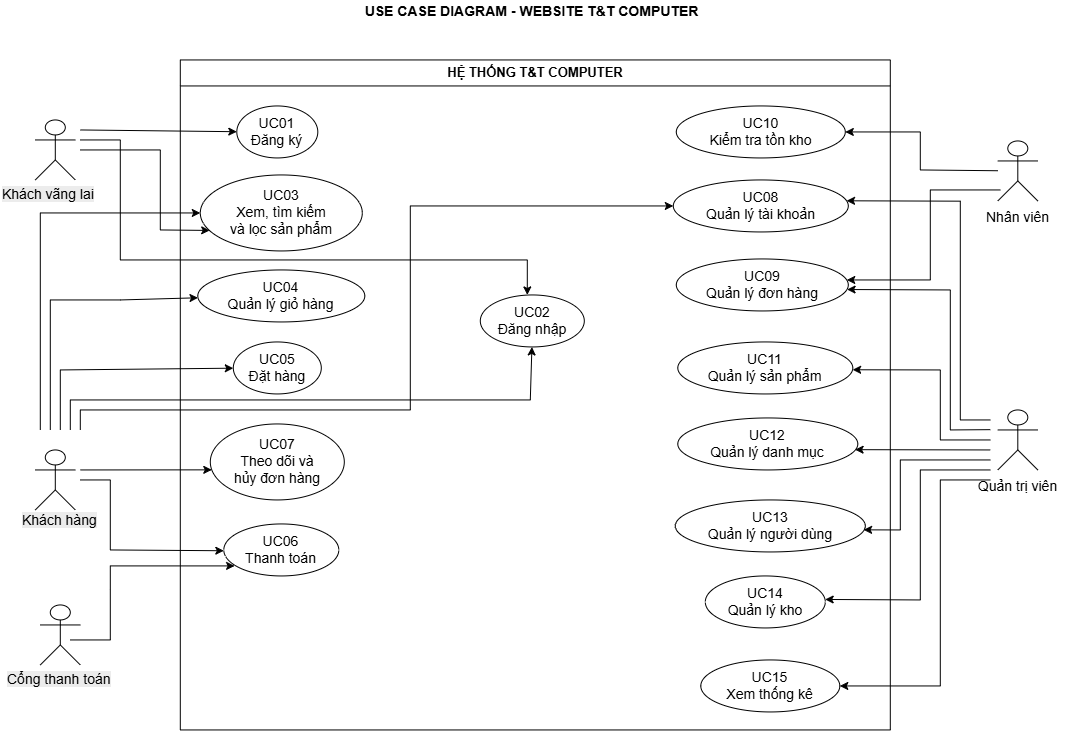
\includegraphics[width=\textwidth]{UseCase.png}}{\fbox{\parbox{0.9\textwidth}{\centering Không tìm thấy tệp UMLtongquat.png}}}

 \caption{Biểu đồ Use Case tổng quát}

 \label{fig:usecase-tongquat}

\end{figure}
\newpage
\section{Biểu đồ Class tổng quát}

Biểu đồ Class tổng quát của hệ thống website T\&T COMPUTER

được sử dụng để mô tả các lớp, thuộc tính, phương thức và mối quan hệ

giữa các lớp trong hệ thống.

\begin{figure}[H]

    \centering

    \IfFileExists{class.png}{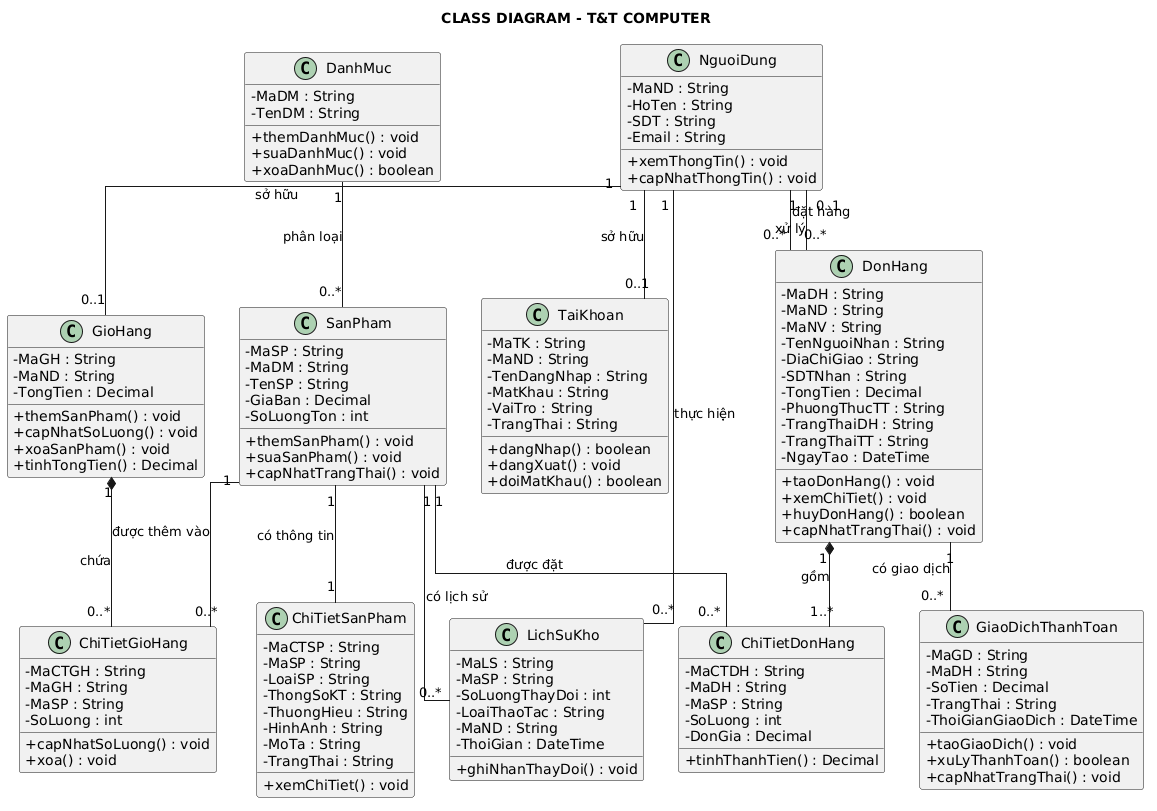
\includegraphics[width=\textwidth]{class.png}}{\fbox{\parbox{0.9\textwidth}{\centering Không tìm thấy tệp class.png}}}

    \caption{Biểu đồ Class tổng quát}

    \label{fig:class-tongquat}

\end{figure}
\newpage
\section{Biểu đồ Database tổng quát}

Biểu đồ Database tổng quát của hệ thống website T\&T COMPUTER

được sử dụng để mô tả các bảng dữ liệu, thuộc tính và mối quan hệ

giữa các bảng trong cơ sở dữ liệu của hệ thống.

\begin{figure}[H]

    \centering

    \IfFileExists{database.png}{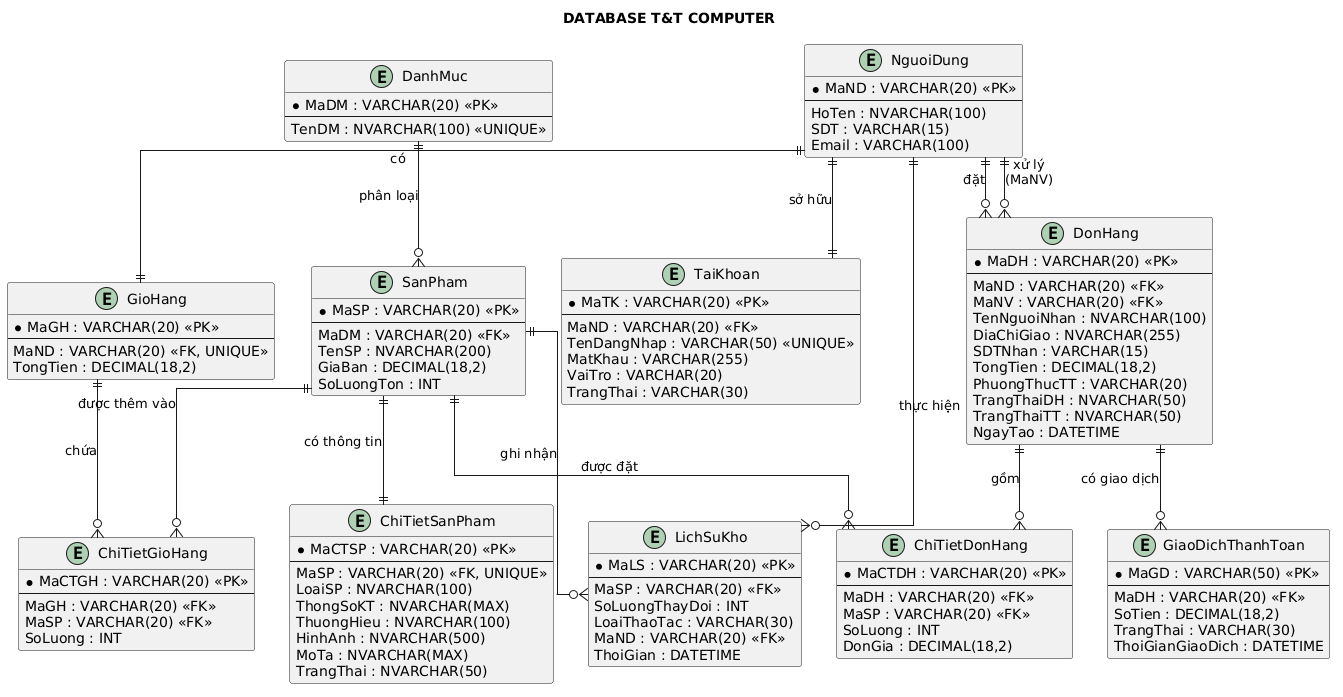
\includegraphics[width=\textwidth]{database.png}}{\fbox{\parbox{0.9\textwidth}{\centering Không tìm thấy tệp database.png}}}

    \caption{Biểu đồ Database tổng quát}

    \label{fig:database-tongquat}

\end{figure}

\end{document}